\chapter{Conclusions}
\label{ch:conclusions}

\section{Summary} % (fold)
\label{sec:exec-sum}
In this thesis I have used near-IR spectroscopic observations to measure the chemical abundance of RSGs in different environments within the Local Universe.
I have detailed the background theory surrounding the evolution of massive stars and their pivotal role in shaping the Universe.
In order to make the best use of the extremely luminous nature of RSGs, I have described and detailed KMOS: the only near-IR multi-object spectrograph in the southern hemisphere.

I have developed and tested a grid-based analysis technique to estimate stellar parameters of RSGs using medium-resolution $J$-band spectroscopy.
I estimate parameters by sampling the posterior probability density function using a maximum-likelihood approach and shown that this technique is not only internally consistent but is also in good agreement with literature measurements.

In Chapter~\ref{ch:ngc2100} this technique is applied to measure the chemistry and kinematics of a YMC in the LMC: NGC\,2100.
KMOS spectra of 14 RSGs in NGC\,2100 are used to estimate the dynamical properties of this star cluster for the first time.
This study demonstrates that KMOS can be used to measure velocities of stars in external galaxies to a precision of $<$5\,\kms and places an upper limit on the line-of-sight velocity dispersion of NGC\,2100 at $\sigma_{1D}$~=~3.9\,\kms, at the 95\% confidence level, where no evidence is found for spatial variations in this estimate.
Using this upper limit, an upper limit to the dynamical mass of NGC\,2100 has been calculated (assuming virial equilibrium) as $M_{dyn}$~=~$15.2\times 10^{4}M_{\odot}$, in good agreement with the literature value of the photometric mass for NGC\,2100.

The chemistry of NGC\,2100 has been estimated using the analysis technique developed in this thesis where the average present-day metallicity of NGC\,2100 is [Z]~=~$-$0.43\,$\pm$\,0.10\,dex, which agrees well with previous studies in this cluster and with studies of the young stellar population of the LMC.

The observational properties of the RSGs in NGC\,2100 are compared with a star cluster of similar age and mass at Solar-like metallicity.
This comparison allows differences in the observational properties of RSGs at different metallicities to be assessed and I show that there appears to be no significant difference between these Solar-like and LMC-like metallicity clusters.

As the RSGs population dominates the infrared light output of a YMC, of a particular age and mass, I combine the RSG spectra to create a simulated integrated-light cluster-spectrum of NGC\,2100.
Using the same analysis technique I demonstrate that the stellar parameters estimated using integrated-light spectroscopy of YMCs are representative of the average parameters of the RSG population within the cluster.

In Chapter~\ref{ch:ngc6822} KMOS spectroscopy of 18 RSGs in the dwarf irregular galaxy NGC\,6822 is presented.
The KMOS data used in this chapter was obtained using KMOS-SV time before this instrument was released to the general community.
This chapter represents the first KMOS study of RSGs and forms the base of which all other studies in this area are built from.
In order to characterise the performance of the data reduction I have reduced and analysed the data using two different methods of telluric correction: the more time expensive 24-arm telluric correction and the more efficient three-arm telluric correction method.
Both methods give consistent results and the 3-arm telluric correction is shown to work as effectively (in most cases).
However, we caution, in the low signal-to-noise regime, the 24-arm telluric method will give more reliable results.

Stellar parameters are calculated using two different analysis techniques and are shown to agree well.
The present day metallicity of NGC\,6822 from RSGs is
[Z]~=~$-$0.55$\pm$0.13\,dex which is consistent with previous measurements of the young stellar population in NGC\,6822.
The data show evidence for a low-significance abundance gradient within NGC\,6822: if real, this would be the first of its kind in a dwarf irregular galaxy.
A larger follow-up study is required in order to fully characterise this gradient.

The chemical abundances of the young and old stellar populations are well explained by a simple closed-box chemical evolution model.
However, while an interesting result, we note that the closed-box model is unlikely to be a good assumption for this galaxy given its morphology.

The effective temperatures of RSGs are compared in four galaxies using the same analysis technique.
These environments span 0.55\,dex in metallicity (Solar to SMC) and no evidence is found for a significant variation in temperature with respect to metallicity.
This is in contrast with evolutionary models which, for a  similar change in metallicity, produces a shift in the temperature of RSGs of up to 450\,K.
In addition, in this chapter I argue that the observed shift in the spectral type of RSGs (defined at optical wavelengths) with respect to metallicity does not imply that the temperatures of RSGs is dependent upon metallicity.


In Chapter~\ref{ch:ngc55} multi-epoch KMOS spectroscopy is presented of 22 RSGs in the Sculptor Group galaxy NGC\,55.
I have measured radial velocities for each epoch which agree well with previous measurements.
All targets with reliable velocities are shown to be consistent with membership of NGC\,55.
In addition I have assessed the radial-velocity variability of each target and find no evidence for any variable sources, which is consistent with all targets being single objects.

Stellar parameters are estimated for a sub-sample of the highest S/N targets and the average metallicity is found to be $-$0.36\,$\pm$\,0.25\,dex, in good agreement with previous results for BSGs.
No evidence is found for spatial variations in metallicity given the present sample, however, I note that this is expected as a result of the combination of the spatial coverage of the sample and the uncertainties in the metallicity parameter.

% section summary (end)

\section{Future Projects} % (fold)
\label{sec:future_projects}

\begin{figure}
 \centering
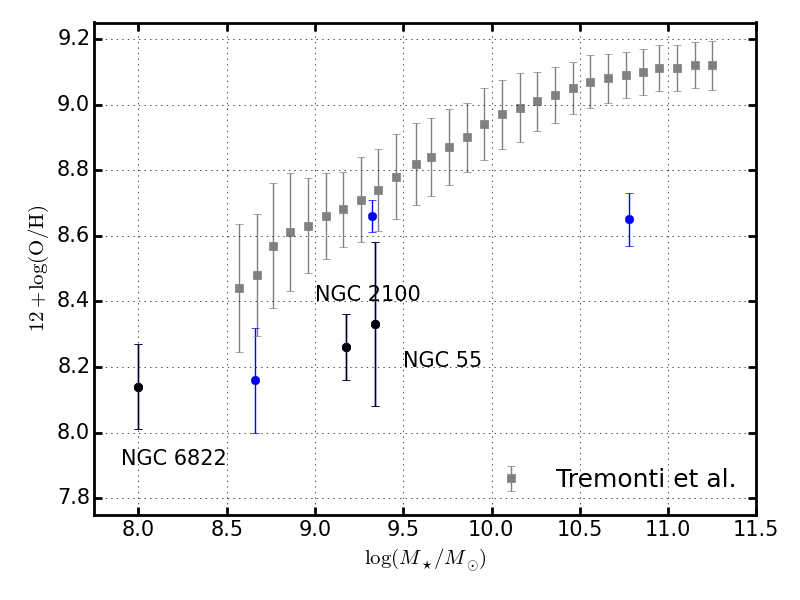
\includegraphics[width=\textwidth]{conclusions/MZR-RSGs}
\caption[Mass-metallicity relation from red supergiant stars]{
The mass-metallicity relation (MZR) for red supergiant stars (RSGs) in the Local Universe shown with blue points where the work included in this thesis is shown with black points.
Metallicity measurements are compiled from the Small Magellanic Cloud
\protect\citep{2015ApJ...806...21D}, Perseus OB-1
\protect\citep{2014ApJ...788...58G}, NGC\,300
\protect\citep{2015ApJ...805..182G},
NGC\,2100 (Chapter~\ref{ch:ngc2100}),
NGC\,6822 (Chapter~\ref{ch:ngc6822})
and NGC\,55 (Chapter~\ref{ch:ngc55}).
By introducing the Solar oxygen abundance ratio~\citep[12 + $\log$ (0/H)$_{\odot}$~=~8.69][]{2009ARA&A..47..481A} I compare these results to the local MZR for galaxies at z~$\sim$~0.1~\citep{Tremonti04}.
This is the first calibration of the MZR using RSGs.
From this figure it is clear that the absolute measurement of metallicity~\citep{Tremonti04} is significantly overestimated, however, to quantitatively assess this relationship requires a larger sample of RSGs in the Local Universe.
\label{fig:concMZR}
         }
\end{figure}

As the topic of this thesis explores many different environments and attempts to relate observations not only to stellar evolution but also to galaxy evolution in general, there are many future projects which build on the present study.
One of the key aims of this thesis has been to develop the use of RSGs as chemical abundance probes in external environments.
Having demonstrated the effectiveness of RSGs as useful tools to measure chemical abundances in a range of galaxies in low-metallicity environments, I can compile an initial calibration of the MZR using the results presented here.

In Figure~\ref{fig:concMZR} I present a first-look at the calibration of the MZR in the Local Universe using RSGs as probes of chemical abundances in external galaxies.
This figure displays results for six galaxies in the Local Universe (blue points) where three of the metallicity measurements have been made in this thesis (black points).
In addition, I show the results of~\cite{Tremonti04} who measured the MZR for $\sim$50\,000 SDSS galaxies in the Local Universe (z~$\sim$~0.1) and by introducing the Solar oxygen abundance ratio~\citep[12 + $\log$ (0/H)$_{\odot}$~=~8.69][]{2009ARA&A..47..481A} I compare these two results.
This figure appears to show a significant offset between the metallicity measurements of these two data sets, however, a larger sample of measurements from RSGs is required to quantitatively assess this offset and differences in these relationships.


To solve this problem of poor sample size I am part of a collaboration which aims to measure chemical abundances from RSGs using techniques developed in this study with KMOS observations of RSGs in 13 galaxies.
This will allow us to provide a full, independent calibration of the MZR using RSGs in the Local Universe.
The observational campaign has been partially successful through use of KMOS GTO and SV data, however, the core proposal for this project was only partially completed in 2015 as a result of poor weather during observing.
I am part of the team that has re-applied for time to observe the final three galaxies in this sample.
When fully complete, this project will allow for the most precise determination of the MZR to date and will provide a foundation for calibration of future extragalactic abundance work.


In addition to the calibration of the MZR which was known to be a project which would greater than the work of one PhD thesis, something which was an unexpected result of this thesis has been the result that there exists no significant variation in the temperature of RSGs with respect to metallicity.
In Figure~\ref{fig:TeffvsZ} I compile all observations of RSGs analysed using the same approach as the one described in this thesis.
This figure shows effective temperature as a function of the metallicity, estimated using the $J$-band analysis technique, for 81 targets in seven different metallicity environments ranging from Solar in PerOB1 to the low-metallicity environment of NGC\,6822 spanning a range of 0.55 dex in metallicity.
The mean of the distribution is 3990\,K with a standard deviation of 150\,K.

\begin{figure}
 \centering
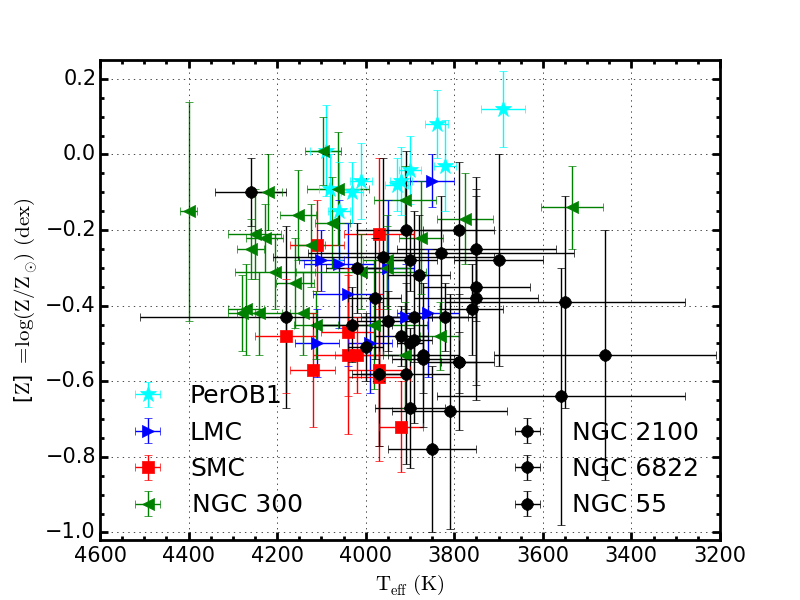
\includegraphics[width=\textwidth]{conclusions/RSGTeffvsZ-all}
\caption[Effective temperature as a function of metallicity in different environments]{
Effective temperatures as a function of metallicity for five different data sets using the $J$-band analysis technique.
There appears to be no significant variation in the temperatures of RSGs over a range of 0.55\,dex.
These results are compiled from the LMC, SMC
\protect\citep[blue and red points respectively;][]{2015ApJ...806...21D}, PerOB1
\protect\citep[a Galactic RSG cluster; cyan;][]{2014ApJ...788...58G} and
NGC\,2100 (Chapter~\ref{ch:ngc2100}),
NGC\,6822 ((Chapter~\ref{ch:ngc6822})
and NGC\,55 ((Chapter~\ref{ch:ngc55}).
The work included in this thesis is shown with black points.
\label{fig:TeffvsZ}
         }
\end{figure}

From this figure I find no evidence for a temperature variation with respect to metallicity.
However, to quantify this fully, a larger sample of RSGs must be studied in a range of different metallicity environments.
Large spiral galaxies are star-forming environments that typically contain hundreds of RSGs and large spatial variations in abundances.
Therefore, a study of a (near) complete population of RSGs in a nearby grand design spiral galaxy e.g. M\,31 or NGC\,300 would be a good starting point to quantitatively assess this interesting result.

In stellar evolutionary models the temperature of RSGs is affected by the choice of the convective mixing length parameter $\alpha_{MLT}$, which is usually fixed at the Solar value ($\alpha$~=~2.0).
A dependence of $\alpha$ on the metallicity of the star could account for the lack of observed temperatures of RSGs.

In Chapter~\ref{ch:ngc6822} I present low-significance evidence for a metallicity gradient within NGC\,6822. Previously in the literature there have been claims for a weak radial metallicity gradient however these claims have been hampered by a lack of precision in metallicity and/or small sample size.
By targeting all candidate RSGs within NGC\,6822 using KMOS GTO in April 2016 I will measure metallicities for $\sim$60 RSG candidates across the full spatial extent of NGC\,6822 (see Chapter~\ref{ch:ngc6822}, Figure~\ref{fig:N6822}).
These follow-up observations will allow me to definitively quantify the spatial distribution of metallicity within NGC\,6822.
This is an important result to quantify as a radial metallicity gradient would be direct evidence for a disk structure in NGC\,6822.

In addition to follow-up spectroscopy in NGC\,6822, our collaboration has re-submitted for KMOS spectroscopy of an additional one field in NGC\,55 to extend the spatial profile covered in this galaxy.
By estimating metallicities for an additional $\sim$20 targets in the disk of NGC\,55 I will be able to more rigorously quantify the abundance gradient in this galaxy with the aim to independently calibrate the metallicity gradient measured from BSGs (Kudritzki et al. in prep.).
In addition to this, by measuring temperatures of the RSGs more accurately in NGC\,55 I will be able to quantify the potential offset in temperatures between this data set and that of NGC\,300.

In Chapter~\ref{ch:ngc2100} I presented the first determination of (an upper limit to) the dynamical mass of NGC\,2100 as well the unresolved line-of-sight velocity dispersion for this cluster.
By obtaining higher resolution spectroscopy of a large sample of stars within this star cluster one could measure the velocity dispersion profile and resolve the line-of-sight velocity dispersion in this cluster.
One of my unanswered questions from the study presented in Chapter~\ref{ch:ngc2100} is: will this star cluster survive or dissolve in the future?
By more accurately determining the mass and velocity dispersion profile of this cluster, this question could be resolved.


In addition to these areas of study mentioned above, I am also interested in further developing the analysis technique presented in Chapter~\ref{ch:janal}.
Studies in this area may include fitting for the [$\alpha$/Fe] parameter (rather assuming Solar-like values), an important indicator of stellar evolution and in particular how this parameter depends upon metallicity.
Expanding the wavelength range used to estimate stellar parameters and including updated line lists would allow one to estimate individual elemental abundances as well as overall metallicity.
A potentially promising channel in this respect is the $\sim$1.0\,$\mu$m region.

Another interesting avenue to explore with this analysis technique would be to expand the parameter space of the model grid to apply this technique to other cool stars e.g. Cepheid variables and red giant stars.


Finally, great progress has been made in recent years using tools which aid the data reduction process in the near-IR e.g. {\sc molecfit, skycorr}.
As near-IR spectroscopy becomes more important in our understanding of astrophysics, these tools will become increasingly relied upon to provide accurate and precise corrections (with the added benefit of significantly boosting observational efficiency)..
In this thesis I have taken the first steps using {\sc skycorr} on KMOS data, where this tool has had great success above what can be achieved neglecting this advanced procedure.
In the future I will supplement this by using {\sc molecfit} to perform telluric correction with the goal of optimising future observing strategies.

% section future_projects (end)

\section{Closing Remarks} % (fold)
\label{sec:closing_remarks}

\ldots over a pint I think!
% section closing_remarks (end)

% \bibliography{../journals,../books}
